%!TEX root = main.tex
\section{Evaluation}
\label{sec:eval}

\subsection{Setup}
\phm{Hardware platform.}
In our testbed experiments, we respectively use Llama3.1-8B~\cite{llama3_1_8b_instruct} and Qwen3-32B~\cite{qwen3_32b} as the LLM backend; the Llama3.1-8B model is deployed on a server equipped with A40-PCIe-48GB GPU, and the Qwen3-32B model is deployed on a server with H800-PCIe-96GB GPU. 
Moreover, we also build a simulator of {up to 64 GPUs} to evaluate the scalability performance of \oursched.


\phm{Workloads.}
In our experiments we use three typical inference datasets as in \cite{hu2024inference}: SharedGPT~\cite{sharegpt_vicuna_unfiltered_2025}, Alpaca-Summarization~\cite{alpaca_pubmed_summarization_2025}, and Document-Write~\cite{write_doc_sft_v1_2025}. 
The characteristics of those datasets are previously elaborated in Fig.~\ref{fig:background_hybridity}. 
Regarding request submission interval, we employ a Poisson distribution under different $\lambda$ hyper-parameters (yielding diverse task rates). 



\phm{Baselines.}
We compare our \oursched solution with multiple representative baselines: FCFS~\cite{kwon2023efficient}, FastServe~\cite{wu2023fast}, SSJF~\cite{qiu2024efficient}, LTR~\cite{fu2024efficient}, and TRIAL~\cite{shahout2024don}.
All of those baselines have been elaborated in Sec.~\ref{subsec:limitations}, and their hyper-parameters are all set as default. 
Besides, by default, for \oursched the selection ratio in predictor is set to 0.8, and the bucket size for Gittins analysis is set to 200. 



\phm{Metrics.}
As elaborated in Sec.~\ref{subsec:problem}, we use the average TTLT 
%(Time to Last Token) 
as the primary scheduling metric.
That said, we also evaluate the average TTFT 
%(Time to First Token) 
performance of each scheduler.


\subsection{End-to-end Experiment}

\begin{figure}[t]
    \centering
    
    \subfigure[Llama3.1-8B]{
        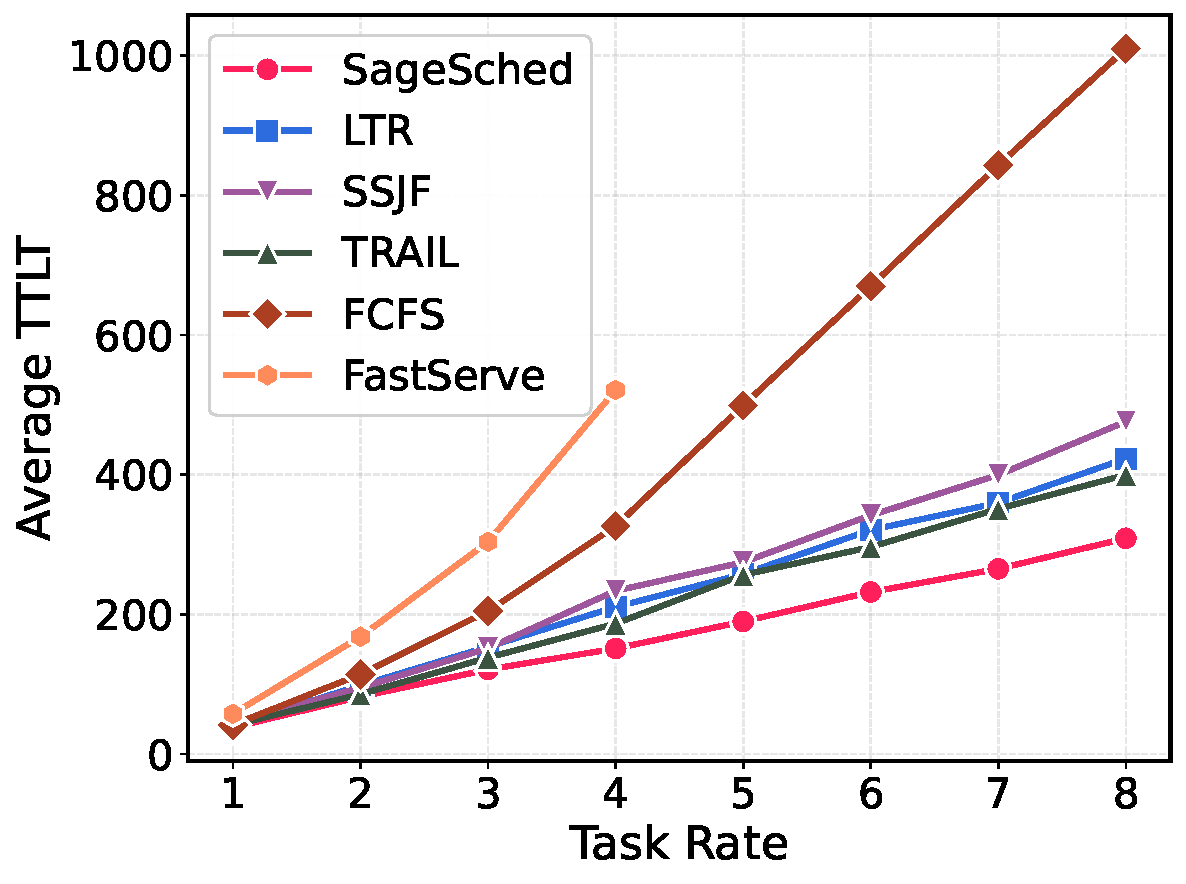
\includegraphics[width=0.45\linewidth]{figures/ttlt_plot_8b.pdf}
        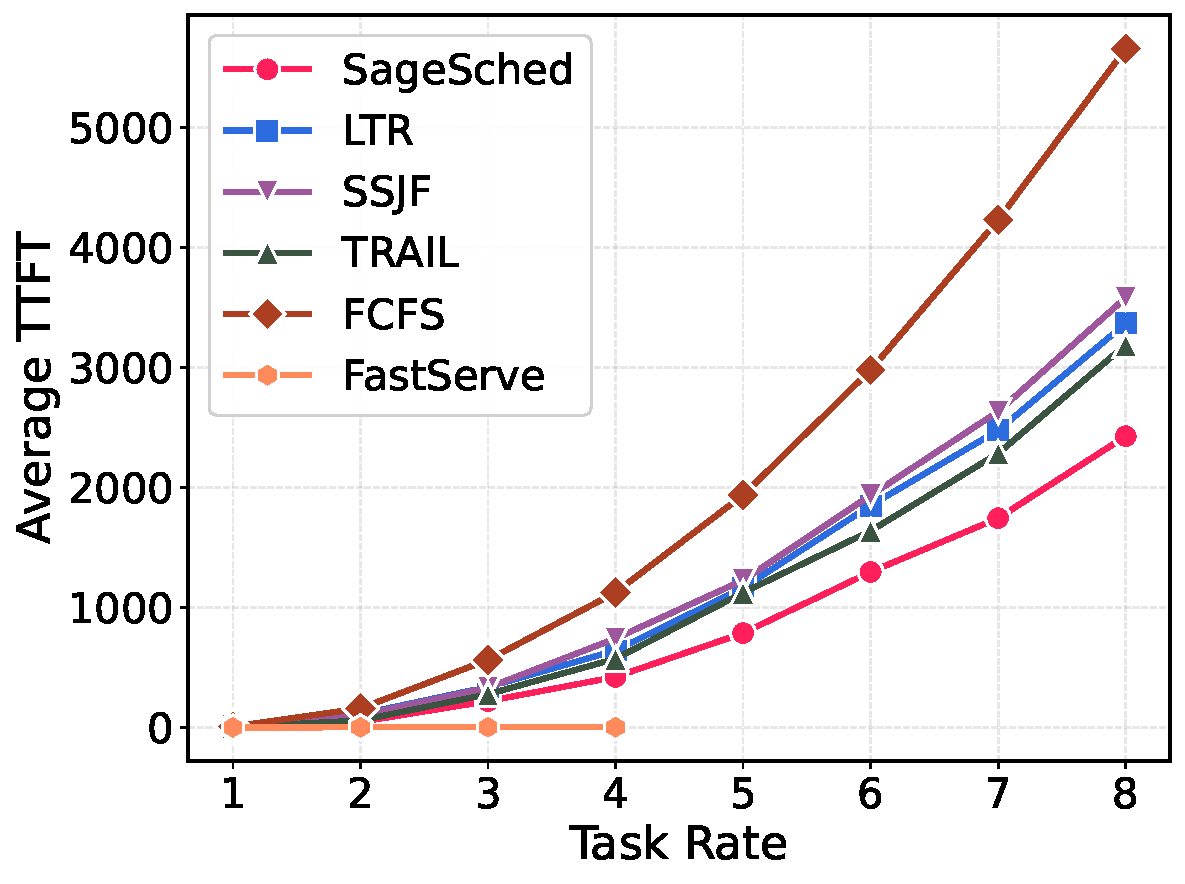
\includegraphics[width=0.45\linewidth]{figures/ttft_plot_8b.pdf}
        \label{fig:e2e 8b ttft}
    }

    \subfigure[Qwen3-32B]{
        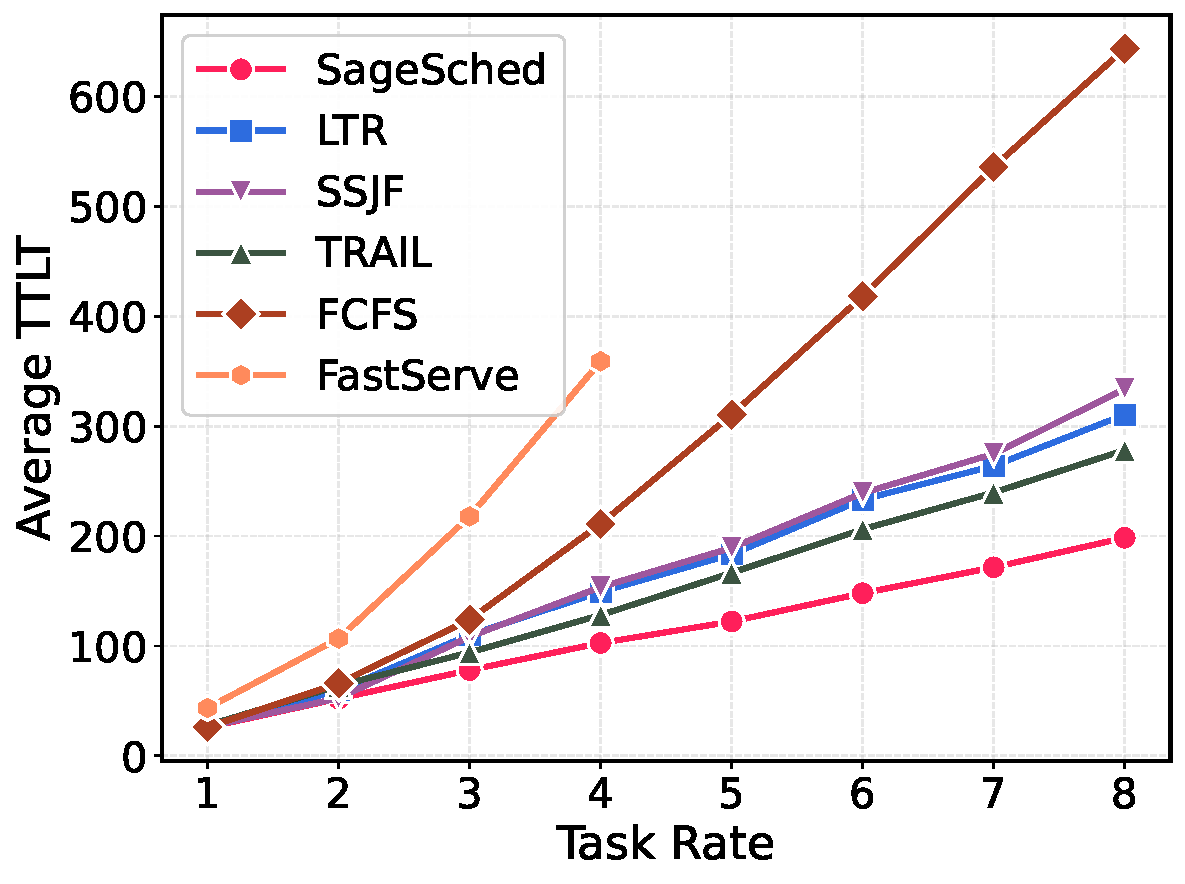
\includegraphics[width=0.45\linewidth]{figures/ttlt_plot_32b.pdf}
        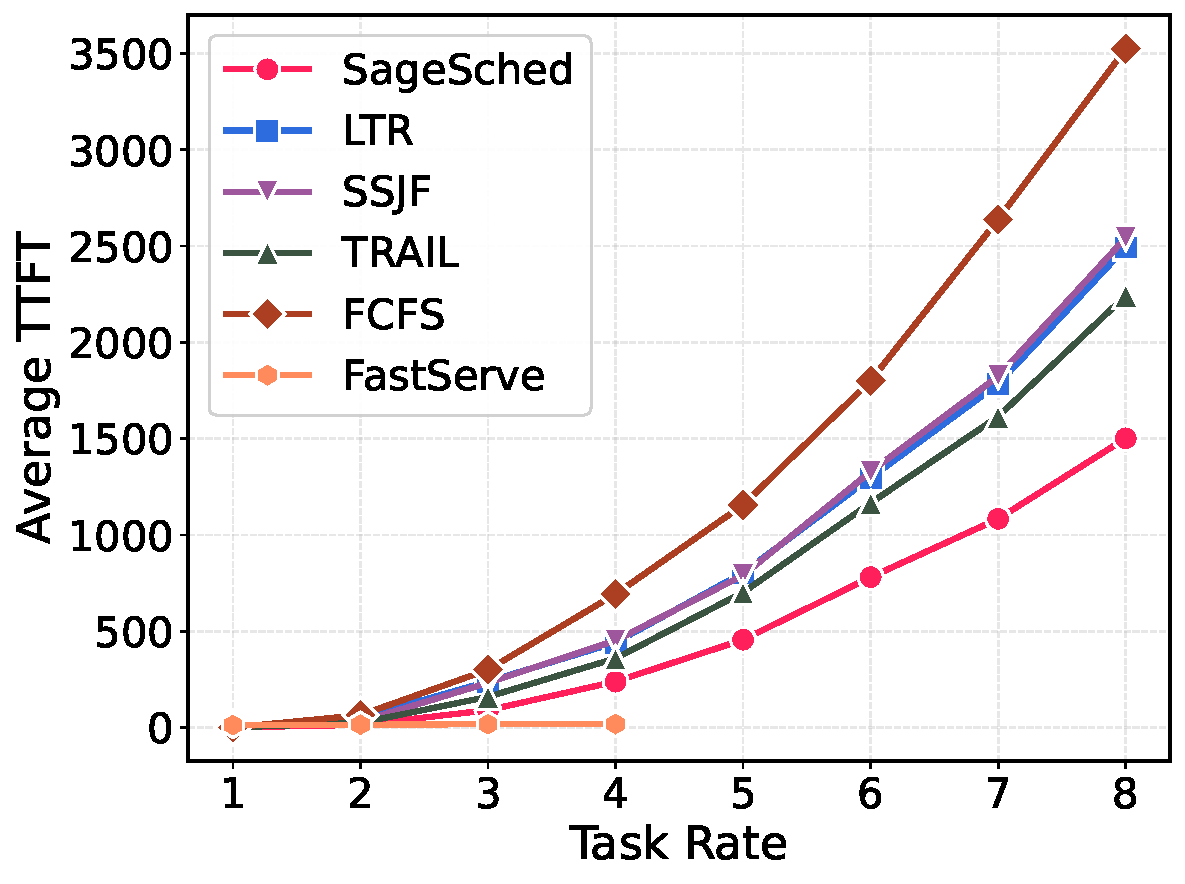
\includegraphics[width=0.45\linewidth]{figures/ttft_plot_32b.pdf}
        \label{fig:e2e 32b ttft}
    }

    \caption{End-to-end performance on mixed datasets.}
    \label{fig:e2e}
\end{figure}

\phm{Experiments with requests from mixed datasets.}
In our end-to-end evaluation, we first merge the three datasets together, the requests from which are then randomly submitted; we experiment respectively
%chosen for submission---respectively at 
under different task rates. 
As shown in Fig.~\ref{fig:e2e}, \oursched demonstrates the best scheduling efficiency in TTLT across all the setups.
For example, when inferences are submitted at a rate of 8 requests-per-second (RPS) to the Qwen3-32B model, \oursched surpasses the second best scheduler, TRAIL, by 28.7\%. 
Such improvements are higher in cases with more intensive competitions, because \oursched can consistently work out the best scheduling order by properly handling the uncertainty and hybridity characteristics of LLM inference demands.
%Such benefits come from the fact that \oursched can effectively address the uncertainty and hybridity characteristics of LLM resource demands.

Regarding TTFT, while it is not the primary focus of this paper, Fig.~\ref{fig:e2e} indicates that \oursched can also attain a satisfying performance, because it can effectively mitigate the head-of-line-blocking problem. 
In particular, although FastServe---by always prioritizing the newly-arrival requests---can attain the best TTFT, in TTLT, it however behaves much worse than other schedulers due to its interleaved execution mode with MLFQ. 
In that sense, \oursched is the only scheduler that can behave well in both TTLT and TTFT. 



\begin{figure}
    \centering
    
\includegraphics[width=1\linewidth]{figures/end_to_end.pdf}
    \caption{End-to-end performance respectively with each dataset.} %\chen{add long/short input/output info? error bars?}}
    \label{fig:single_dataset}
\end{figure}

\phm{Experiments with request respectively from each dataset.}
Recall that the three datasets we use have different input-output length distribution (Fig.~\ref{fig:background_hybridity}); we thus experiment respectively with each dataset, with the results shown in Fig.~\ref{fig:single_dataset}.
We first note that \oursched consistently perform the best for each dataset.
In particular, its performance superiority peaks for the Alpaca (Summarization) dataset: this is because requests in Alpaca dataset typically have long input lengths, for which existing output-length based scheduling methods are highly inaccurate in cost modeling. 



\subsection{Microscopic Deep Dive}

In this part, we dive deep into the effectiveness of each solution component in \oursched.
Unless otherwise specified, we use the same setup as in Fig.~\ref{fig:e2e} (under a RPS of 8).

\subsubsection{Superiority of our Predictor Design}

Given the deficiency of conventional output-length predictors, in Sec.~\ref{subsec:predictor} we propose a novel \emph{semantic-aware history-based predictor}.
Here we check its necessity with regard to the end-to-end TTLT performance.
Specifically, we incorporate two baselines representing the other prediction choices: (1) \emph{semantic-unaware history-based predictor}---which predicts the output-length length of a request by referring to the historical requests with a similar input length (following the same filtering method as us), and (2) \emph{semantic-aware LLM-based predictor}---still using a DistillBert model as in \cite{qiu2024efficient} yet, to predict a distribution, we remove the \texttt{logits.argmax} layer.
In Fig.~\ref{fig:ablation_prediction}, we show the performance of \oursched respectively with different predictors.
It shows that with our semantic-aware history-based predictor, due to its high distribution-prediction accuracy, \oursched can make the best TTLT performance.

Moreover, we note that our predictor also surpasses others in training and prediction overheads.
First, our method completely eliminates training overhead, whereas for the LLM-based predictor, it takes several hours to construct a training dataset and also tens of minutes to perform model fine-tuning.
Second, the average per-request prediction latency is below 0.5 ms under our predictor (consisting of 0.22 ms for semantic embedding extraction and 0.15 ms for vector retrieval), yet for the LLM-based predictor it is approximately 3.6 ms.
Those results above jointly confirm that our semantic-aware history-based predictor is light-weight and also accurate.



\begin{figure}
    \centering
    \begin{minipage}[t]{0.47\linewidth}
        \centering
        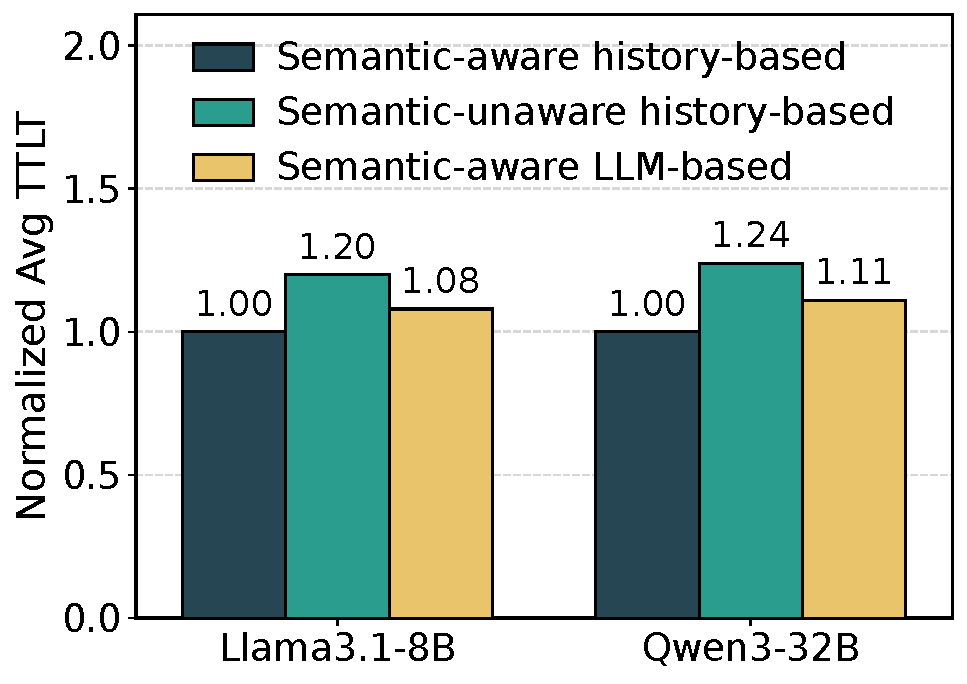
\includegraphics[width=\linewidth]{figures/ablation_on_influence.pdf}
        \caption{Performance comparison of different output-length prediction methods.} %Ablation study on the influence of the method to get output length distribution.}
        \label{fig:ablation_prediction}
    \end{minipage}
    \hfill
    \begin{minipage}[t]{0.47\linewidth}
         \centering
        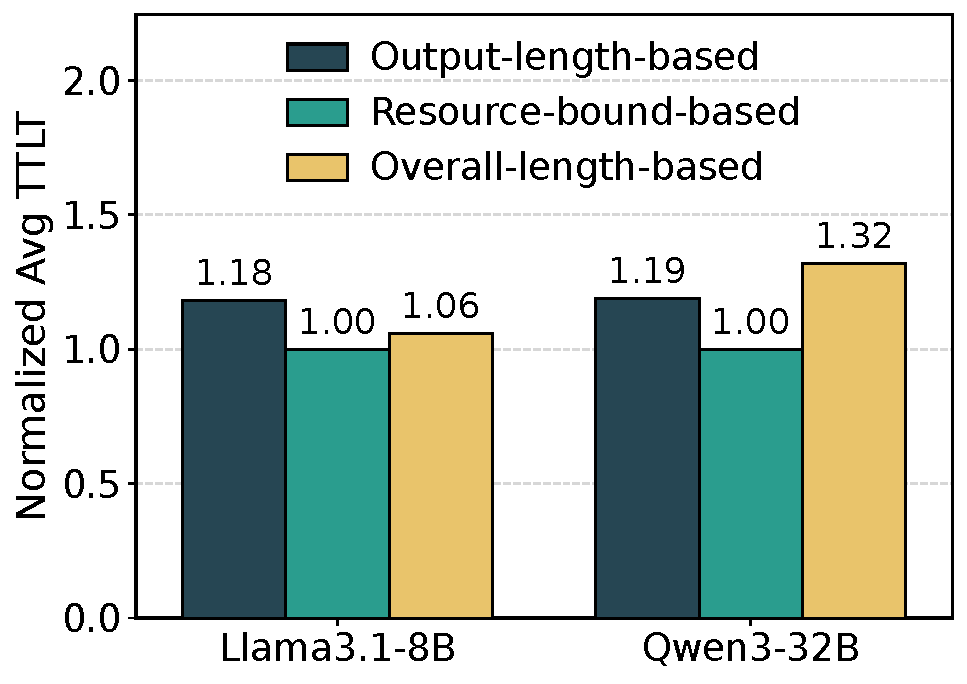
\includegraphics[width=\linewidth]{figures/ablation_on_cost.pdf}
        \caption{Performance comparison of different service cost modeling methods.}
        \label{fig:ablation_cost}
    \end{minipage}
    \hfill
\end{figure}



\subsubsection{Superiority of our Cost Modeling Method}
\label{sec:cost modeling}


In Sec.~\ref{subsec:cost}, after analyzing both the compute- and memory-bound cases,
%by respectively analyzing the compute-bound and memory-bound cases,
we developed a \emph{resource-bound-based modeling} method to depict LLM inference cost.
%: $\mathcal{C}=\frac{O^2}{2}+IO$.
To confirm its necessity, we replace it respectively to two other methods: (1) \emph{output-length-based modeling}---which directly uses the output length as the inference cost~\cite{shahout2024don,qiu2024efficient}, and (2) \emph{overall-length-based modeling}, which combines the input and output lengths as the cost (we assign the output length a doubled weight as in \cite{sheng2024fairness}). 
Fig.~\ref{fig:ablation_cost} shows the overall TTLT performance under different modeling methods. % (with the other setups resembling Fig.~\ref{fig:ablation_prediction}).
It confirms the necessity to adopt the resource-bound-based method for cost modeling. 


\subsubsection{Superiority of our Scheduling Policy}
%\chen{mean vs. mean+error vs. mean (runtime update) vs. mean (runtime update) + error + gittins vs. gittins+error}

Recall that our uncertainty-aware scheduling algorithm in Sec.~\ref{subsec:gittins} has two key techniques: 
\emph{Gittins-index-based ordering}, and \emph{runtime Gittins-index refreshing}.
Here we respectively evaluate the benefit of each technique; besides, we also need to check the robustness of scheduling quality in cases with inaccurate predictions.
Specifically, we first introduce two additional baselines: (1) \emph{Mean}---which orders requests based on the \emph{mean} value of their cost distributions, and (2) \emph{Gittins}$-$---which applies the Gittins policy but without timely refreshing the Gittins index at bucket boundaries.
Moreover, for each scheduler, we also measure its performance against \emph{inaccurately-predicted} cost distributions (by merging a \emph{uniform} distribution to the original distribution following a weight ratio of 1:4). 
As shown in Fig.~\ref{fig:ablation_gittins}, both Gittins-index-based ordering and runtime Gittins-index refreshing are beneficial for TTLT performance; besides, the added noises incur much less performance degradation to our Gittins-index-based algorithm than to other baselines.


% \begin{figure}
%     \centering
%     \includegraphics[width=0.6\linewidth]{figures/ablation_gittins.pdf}
%     \caption{Sensitive study on the effect of how to utilize the output length distribution}
%     \label{fig:sensitive}
% \end{figure}
\begin{figure}[t]
    \centering
    \begin{minipage}[t]{0.47\linewidth}
        \centering
        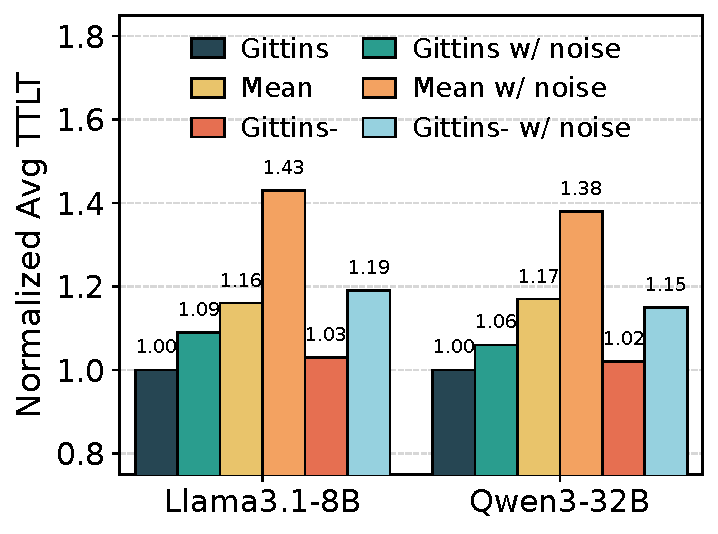
\includegraphics[width=\linewidth]{figures/ablation_on_effect.pdf }
        \caption{Comparison of different scheduling methods, even with added cost noises.} % Ablation study on the effect of how to utilize the output length distribution.}
        \label{fig:ablation_gittins}
    \end{minipage}
    \hfill
    \begin{minipage}[t]{0.47\linewidth}
        \centering
        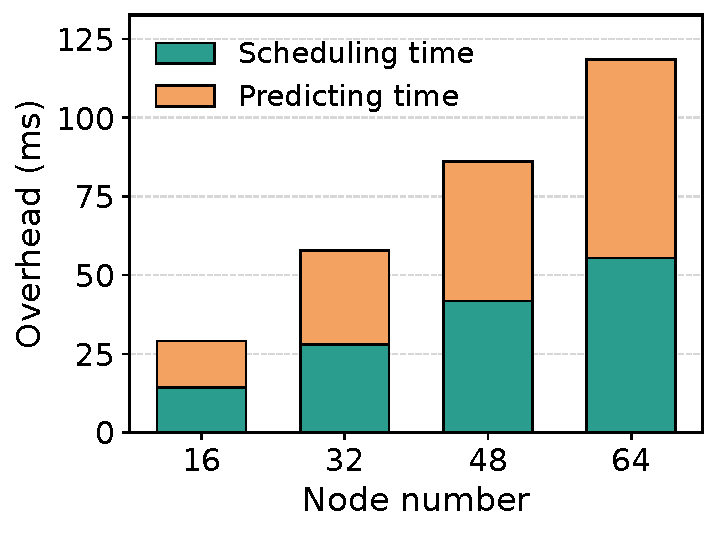
\includegraphics[width=\linewidth]{figures/overhead.pdf}
        \caption{Predicting and scheduling overheads of \oursched at different scales.} %Overhead analysis results}
        \label{fig:overhead}
    \end{minipage}
    
\end{figure}



\subsection{Overhead and Sensitivity Analysis}
\label{subsec:eval_sensitivity}
% \begin{figure}
%     \centering
%     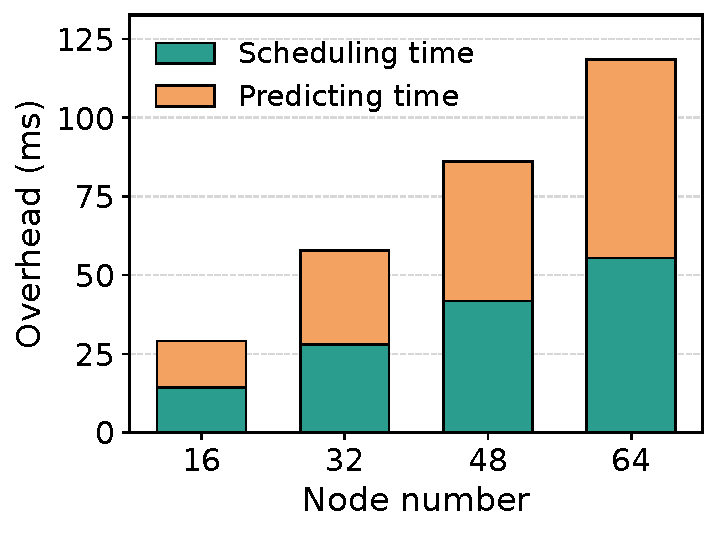
\includegraphics[width=1\linewidth]{figures/overhead.pdf}
%     \caption{Overhead analysis results}
%     \label{fig:overhead}
% \end{figure}

In this part we study the scalability issue of \oursched and also make sensitivity analysis on the hyper-parameters introduced. 
Unless otherwise specified, we also use the same setup as in Fig.~\ref{fig:e2e}. 

%\chen{to revise}\gan{overhead analyz}
\phm{Scalability performance.}
To evaluate the scalability performance of \oursched, we simulate large-scale cluster deployments with up to 64 GPU nodes. 
The system load (RPS) is increased proportionally with the cluster size.
%following a doubling pattern in both concurrency and workload. 
On average, each node serves 8 requests per second (RPS), with up to 1,000 requests buffered in the queue.
We measure the per-request latency incurred during the predicting and scheduling stages, assuming a fixed output length of 1,000 tokens. 
As shown in Fig.~\ref{fig:overhead}, the latency grows only linearly as the cluster scales. 
Even at the largest scale of 64 nodes, the average additional latency per request remains around 100 ms.
Given that typical LLM inference workloads operate at the granularity of several seconds to minutes (as in Fig.~\ref{fig:e2e}), this overhead is indeed negligible.
%demonstrating that our approach scales efficiently to large clusters.
Moreover, for large clusters, we can deploy multiple concurrent schedulers to further alleviate such overhead. 


\phm{Similarity threshold.} 
In predictor design (Sec.~\ref{subsec:predictor}) we adopt a cosine-similarity threshold in filtering out the historical requests with similar prompts. %referable 
Here we respectively set it to different values, with the testbed performance shown in Fig.~\ref{fig:sensitivity_predictor}.
The results confirm that setting it to 0.8 yield the best performance---an over-large threshold renders the selected requests less abundant (compromising the capturing of demand uncertainty), yet an over-small threshold would pollute the sampled distribution with irrelevant requests.

\phm{Bucket size.}
Meanwhile, in Sec.~\ref{subsec:gittins} we also adopt a bucket-size hyper-parameter to control the refreshing frequency of Gittins index. 
As in Fig.~\ref{fig:sensitivity_gittins}, we measure the average TTLT under \oursched with different bucket sizes.
It suggests that a bucket size of 200 can yield the best performance (which we thus adopt as default): smaller bucket sizes lead to more priority calculation and re-scheduling overheads, yet larger bucket sizes compromise the accuracy of priority assignment; both degrade the overall efficiency. 



\begin{figure}[t]
    \centering
    \subfigure[Predictor hyperparameter]{
        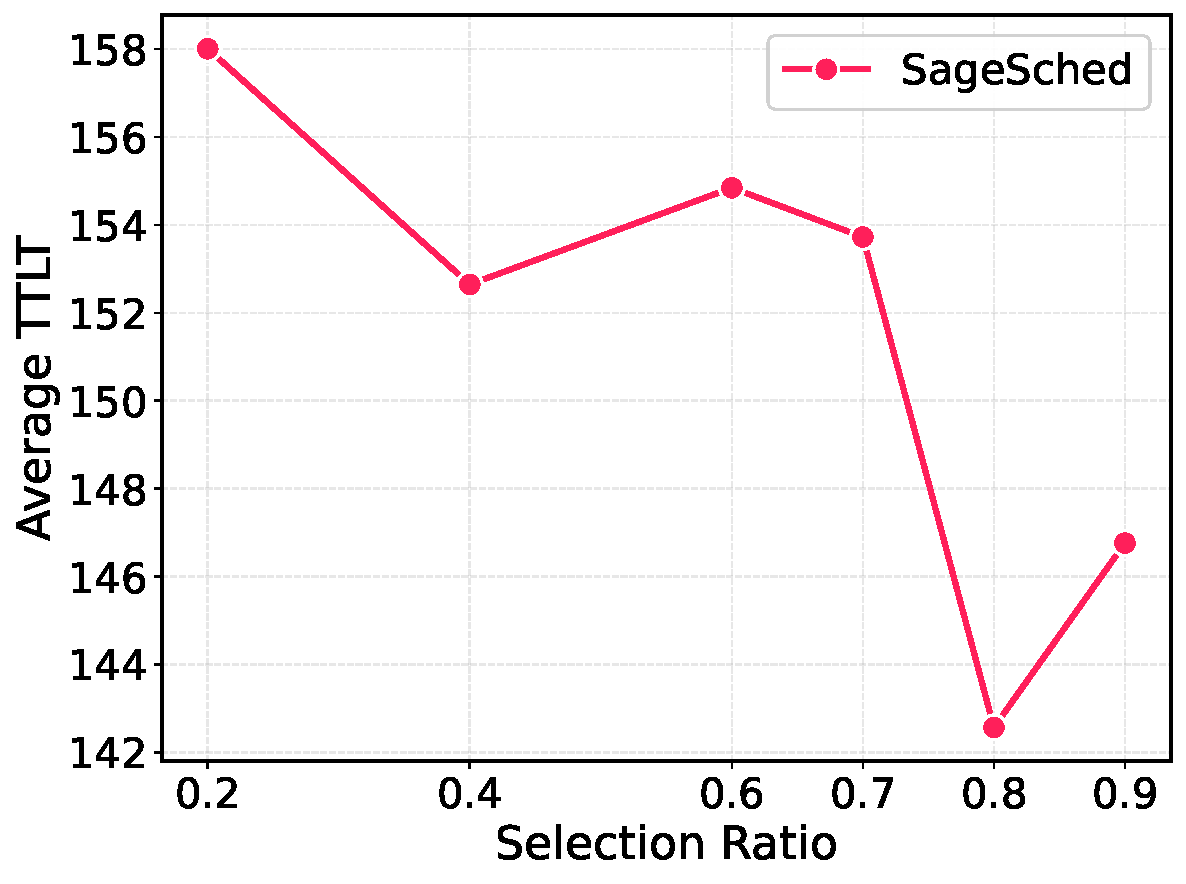
\includegraphics[width=0.45\linewidth]{figures/sensitive_selection.pdf}
        \label{fig:sensitivity_predictor}
    }
    \hfill
    \subfigure[Scheduler hyperparameter]{
        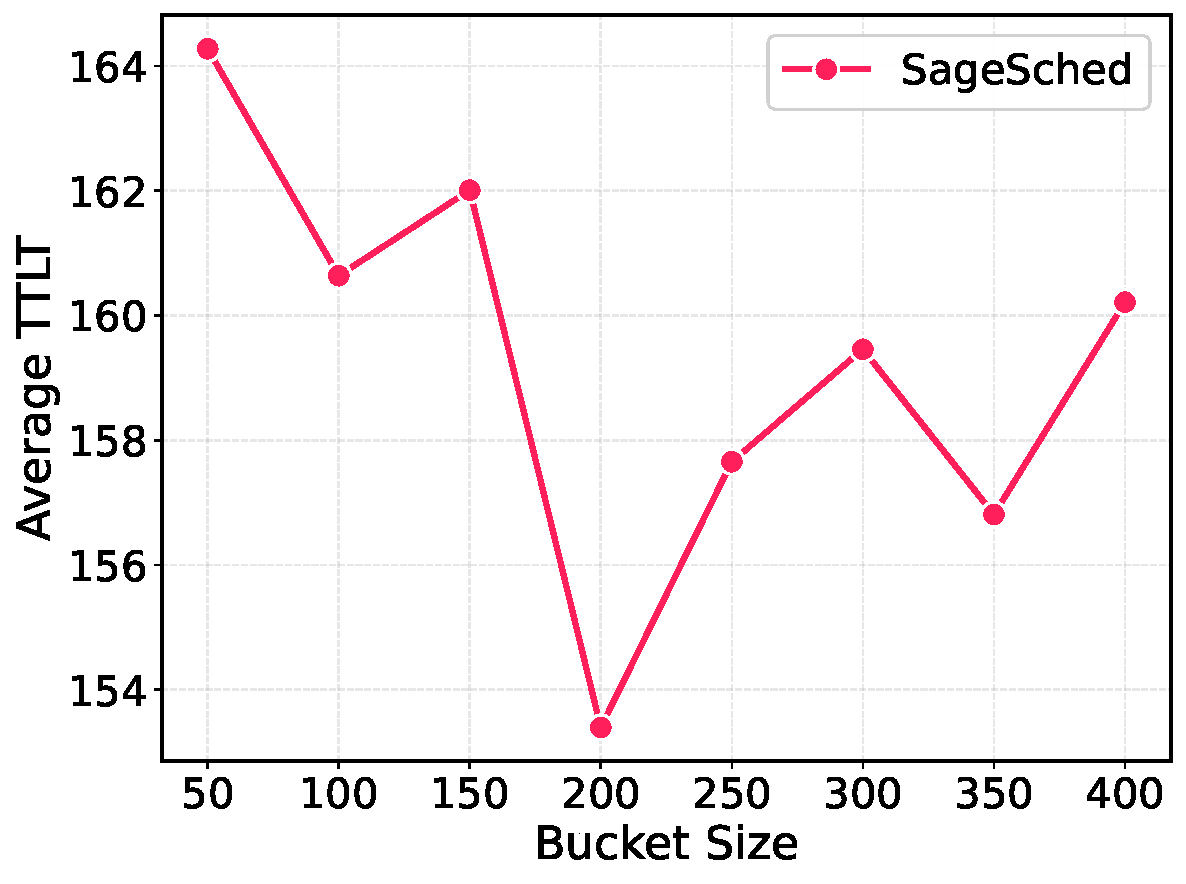
\includegraphics[width=0.45\linewidth]{figures/sensitive_bucket.pdf}
        \label{fig:sensitivity_gittins}
    }
    \vspace{-.1in}
    \caption{Sensitivity analysis of \oursched hyperparameters.}
    \label{fig:sensitivity}
\end{figure}

